\documentclass[newPxFont,numfooter,sectionpages]{beamer}
\usepackage[utf8]{inputenc}
\usetheme{sthlm}
\usepackage[round]{natbib}
\bibliographystyle{plainnat}
\usepackage{amsmath}
\usepackage{amssymb}
\usepackage{amsthm}
\usepackage{dsfont}
\usepackage{hyperref}
\usepackage{multirow}
\usepackage{color}
\usepackage{tikz}
\usepackage{graphicx}
\usepackage{setspace}
\usepackage{bigints}
\usepackage{algorithm2e}
\usepackage{float}
\usepackage{lscape}
\usepackage{rotating}
\usepackage{longtable}
\usepackage[normalem]{ulem}
\hypersetup{
    colorlinks=true,
    linkcolor=black,
    filecolor=magenta,
    urlcolor=blue,
    citecolor=black,
}

\newcommand{\indep}{\mathrel{\text{\scalebox{1.07}{$\perp\mkern-10mu\perp$}}}}
\DeclareMathOperator*{\argmin}{arg\,min}
\DeclareMathOperator*{\argmax}{arg\,max}
\newcommand{\E}{\mathbb{E}}
\newcommand{\V}{\mathbb{V}}
\newcommand{\I}{\mathbb{I}}
\newcommand{\com}[1]{&&\mbox{(#1)}}
\newcommand{\bt}{\mathbf{t}}
\newcommand{\bT}{\mathbf{T}}
\newcommand{\Gnit}{G_{\mathcal{N}_i}^\bt}
\newcommand{\Gnjt}{G_{\mathcal{N}_j}^\bt}
\newcommand{\btheta}{\boldsymbol{\phi}}

\title{Almost-Matching-Exactly for Treatment Effect Estimation under Network Interference}
\subtitle{}
\author{Usaid Awan, Marco Morucci, Vittorio Orlandi}

%\institute{Duke University}
\date{}
\begin{document}
\setbeamercolor{background canvas}{bg=dukeBlue}
\setbeamercolor{title}{fg=white} \setbeamercolor{subtitle}{fg=white}
\setbeamercolor{institute}{fg=white}
\setbeamercolor{author}{fg=white}
\setbeamercolor{normal text}{fg=white}
\maketitle

\setbeamercolor{background canvas}{bg=white}
\setbeamercolor{frametitle}{bg=dukeBlue}
\setbeamercolor{normal text}{fg=sthlmDarkGrey, bg=sthlmGrey}

\begin{frame}{Setting - Causal Inference}
\begin{itemize}
  \item We have $i=1, \dots, n$ experimental units
  \item Treatment $t_i \in \{0, 1\}$ with $\bt \in \{0, 1\}^n$ is a binary vector with the treatment level of every unit.
  \item Potential outcomes $Y_i(t_i, \bt)$ are random variables and depend on both treatment of unit $i$ (1st argument), and treatment of \textbf{all other units} (2nd argument).
  \item Observed treatment $\bT \in \{0, 1\}^n$ is assigned \textbf{uniformly at random}.
  \item Observed outcome: $Y_i = T_iY(1, \bT) + (1-T_i)Y_i(0, \bT)$
  \begin{itemize}
    \item Since treatment is randomized: $\E[Y_i|\bT = \bt, T_i = t] = \E[Y_i(t, \bT)]$ (Ignorability).
  \end{itemize}
  \item Units are connected in a network, $G$, in which unit $i$'s \textbf{treated neighborhood subgraph} is $\Gnit$.
\end{itemize}
\end{frame}

\begin{frame}{The Problem: No SUTVA!}
Usually we assume SUTVA: that \textit{units' treatments don't influence other units' outcomes}, but we can't do that here because our units are connected in a network:
\begin{center}
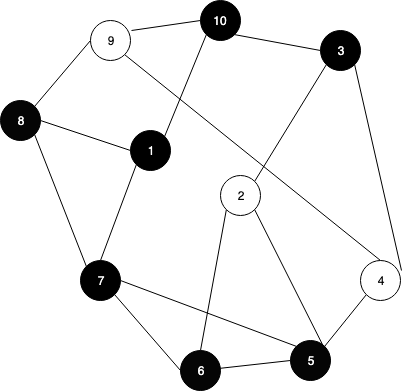
\includegraphics[height=1.8in]{graph1.png}
\end{center}
It could be that the treatment assigned to $j$ influences the outcome of $i$ through their connection in the network.
\end{frame}

\begin{frame}{Similar Graphs Carry Similar Interference}
\begin{alertblock}{Idea}
What if the amount of interference experienced by a unit depended on the \textit{shape} of its treated neighborhood subgraph?
\end{alertblock}
\begin{center}
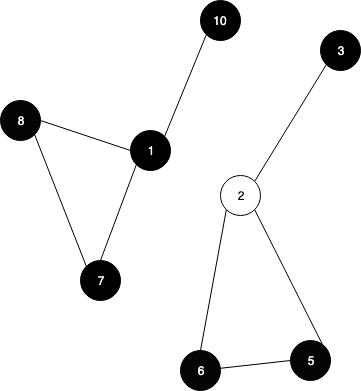
\includegraphics[height=1.5in]{graph2.png}
\end{center}
Then, in expectation, two units with the same treated neighborhood graph will respond similarly to the treatment. \\
\textbf{We can use this idea to do matching to reduce interference.}
\end{frame}

\begin{frame}{Assumptions}
\begin{enumerate}
  \item Outcome model: $Y_i = \alpha + t_i\beta_i + f_i(\Gnit) + \epsilon_i$
  \begin{itemize}
    \item $f$ is some interference function dependent on $\Gnit$, the \textbf{treated neighborhood subgraph} of unit $i$.
  \end{itemize}
  \item $\E[\epsilon_i|T_i] = \E[\epsilon_i] = 0$
    \begin{itemize}
    \item Ignorability
  \end{itemize}
  \item If $\Gnit \simeq \Gnjt$ then $f_i(\Gnit) = f_j(\Gnjt) = f(\Gnit)$.   \begin{itemize}
    \item Two units with isomorphic neighborhood sugraphs experience the same interference.
    \item Together with (1), this assumption encodes a version of SANIA (Airoldi and Sussman, 2018) conditional on unit's neighborhood subgraphs.
  \end{itemize}
\end{enumerate}
\end{frame}
\begin{frame}{Matching}
\begin{itemize}
  \item Under these assumptions we can match units to recover the effect we are interested in ($\tau_i$)
  \item For a treated unit $i$, find a control unit $j$, such that $\Gnit \simeq \Gnjt$
  \item Subtract $Y_j$ from $Y_i$ to recover $\tau_i$ in expectation
\end{itemize}
\begin{align*}
\E[Y_i - Y_j] &= \E[\tau_i + f(\Gnit) - f(\Gnjt) + \epsilon_i + \epsilon_j] = \tau_i
\end{align*}
If no unit has exactly $\Gnjt \simeq \Gnit$ we can find a unit that has a neighborhood graph that is not quite equal to $\Gnit$ but is similar enough.
\begin{alertblock}{Problem}
How do we represent similarity between neighborhood graphs?
\end{alertblock}
\end{frame}
\begin{frame}{Subgraph Counts}
	\begin{itemize}
		\item We'll say that neighborhood graphs are similar if they contain similar counts of subgraphs
    \item In fact, if the counts of subgraphs are the exact same, then the neighborhood graphs must be isomorphic.
    \item We match together units that have the most similar subgraphs
    \item If no unit matches exactly to another on all subgraph counts, then we must choose which subgraphs we want to match exactly on and which ones we can afford to ignore.
	\end{itemize}
\end{frame}
\begin{frame}{Subgraph Counts}
\begin{center}
  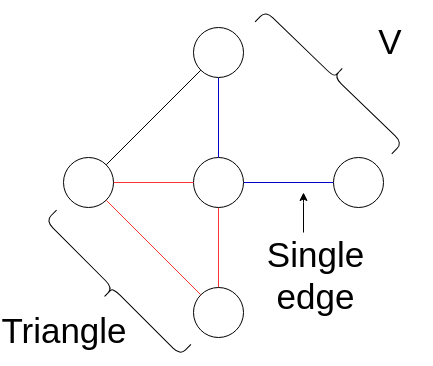
\includegraphics[width=0.7\linewidth]{subgraphs.png}
\end{center}
This graph has 2 triangles, 6Vs and 4 single edges.
\end{frame}
\begin{frame}{$\cdot$AME-Networks}
\begin{alertblock}{Problem \#2}
How do we choose which subgraphs we should use to represent the treated neighborhood graphs of our units?
\end{alertblock}
\textbf{We need a matching method that \textbf{selects} which subgraphs to match on}
\begin{enumerate}
  \item Enumerate (up to isomorphism) all $p$ subgraphs $S_1, \dots, S_p$ seen across all the $\mathcal{N}_i, i = 1, \dots, n$
  \item For each unit $i$, define the $p$-dimensional vector $S(G_{\mathcal{N}_i^{\mathbf{t}}})$ as the vector whose $j$'th entry is the number of $S_j$ in $\mathcal{N}_i$
  \item These are likely a lot (maximum on the order of $|\mathcal{N}_i|^2$) and it's unlikely that many units will have identical counts
  \item The FLAME matching algorithm will automatically select the best subgraphs to match on
\end{enumerate}
\end{frame}
\begin{frame}{FLAME: An Overview}
	\begin{itemize}
		\item FLAME (Fast Large-Scale Almost Matching Exactly) is a method for creating interpretable matches between units with discrete covariates that performs variable selection while matching.
		\begin{enumerate}
			\item Match units exactly on as many covariates as possible
			\item Drop a covariate
			\item Repeat
		\end{enumerate}
		\item At each step, drop the covariate maximizing match quality:
		\[\mathtt{MQ} = C \cdot \mathtt{BF} - \mathtt{PE}\]
		\item $\mathtt{BF} = $ prop. controls matched + prop. treated matched
		\item $\mathtt{PE} = $ prediction error achieved by remaining covariates
		\item Tradeoff between making matches and accurate prediction
	\end{itemize}
\end{frame}
\begin{frame}{A Small Change to FLAME}
We know from our theoretical setup that network statistics should do two things well:
\begin{enumerate}
  \item Predict the \textbf{outcomes}
  \item Predict the \textbf{network}
\end{enumerate}
To measure how well the our network statistics (subgraphs) are predicting the network, we model the edges of the network as independent conditional on the observed statistics
\[E_{ij}|x_i, x_j \stackrel{iid}{\sim} \textrm{Bern}(\textrm{logit}(\beta_1'x_i + \beta_2'x_j))\]
and consider the AIC of the resulting model, $\text{AIC}_{\text{network}}$.
\end{frame}

\begin{frame}{The Modified $\mathtt{PE}$ Function}
	To ensure FLAME strikes a balance between predicting both the \textbf{outcomes} and the \textbf{network}, we modify the $\mathtt{PE}$ function:
\begin{align*}
	{\tt PE} &= \sum_{t = 0}^1\argmin_{f \in \mathcal{F}}\frac{1}{n}\sum_{i = 1}^n(Y_i - f(S(\Gnit)))^2\\
         &- \underbrace{D\cdot \text{AIC}_{\text{network}}}_{\text{new component}}
\end{align*}
\end{frame}

\begin{frame}{Simulation Setup}
	\begin{itemize}
		\item Recall the outcome model: $Y_i = \alpha + \beta_i t_i + f(G_{\mathcal{N}_i^\mathbf{t}}) + \epsilon_i$
		\item The graph $G$ is generated according to Erdos-Renyi or Stochastic Block models
		\item We consider various forms of $f$ based off different features:
		\begin{itemize}
			\item $d_i$: the degree of unit $i$
   			 \item $\Delta_i$: the number of triangles in $\mathcal{N}_i$
   			 \item $\dagger_i^k$: the number of units in $\mathcal{N}_i$ with degree $\geq k$
 			 \item $\bigstar_i^k$: the number of $k$-stars in $\mathcal{N}_i$
   			 \item Betweenness$_i$: the vertex betweenness of unit $i$
    			\item Closeness$_i$: the closeness centrality of unit $i$
		\end{itemize}
	\end{itemize}
\end{frame}
\begin{frame}{Estimators}
	\begin{itemize}
		\item True: nearest neighbor (NN) on true interference
		\item Naive: naive difference in means
		\item Eigen All: NN on eigenvalues of adjacency matrix $A$
		\item Eigen All: NN on largest eigenvalue of $A$
		\item Stratified Naive: Stratified degree estimator
		\item SANIA: MIVLUE under SANIA
		\item FLAME: Our approach
	\end{itemize}
\end{frame}
\begin{frame}{(OLD) Simulation Results}
\centering
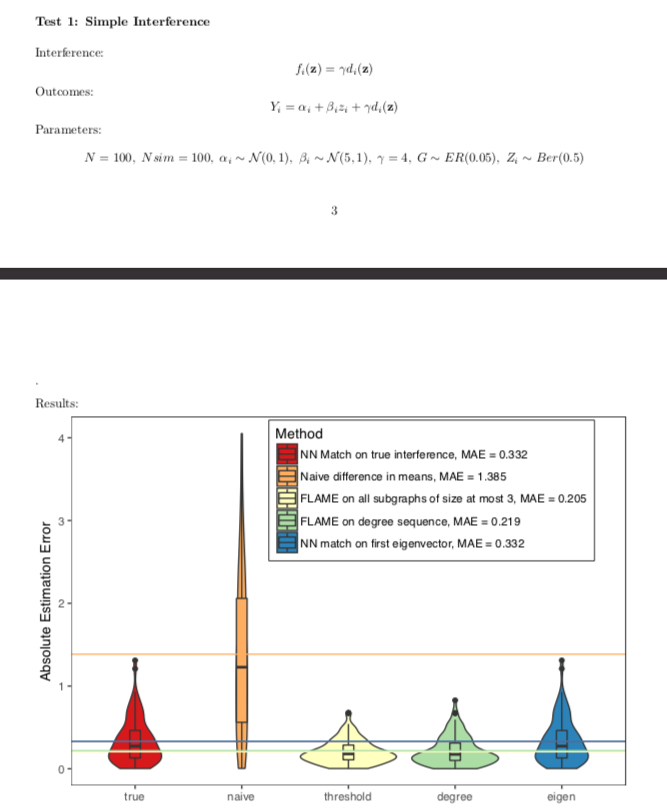
\includegraphics[height=3in]{simple.png}
\end{frame}
\begin{frame}{(OLD) Simulation Results}
\centering
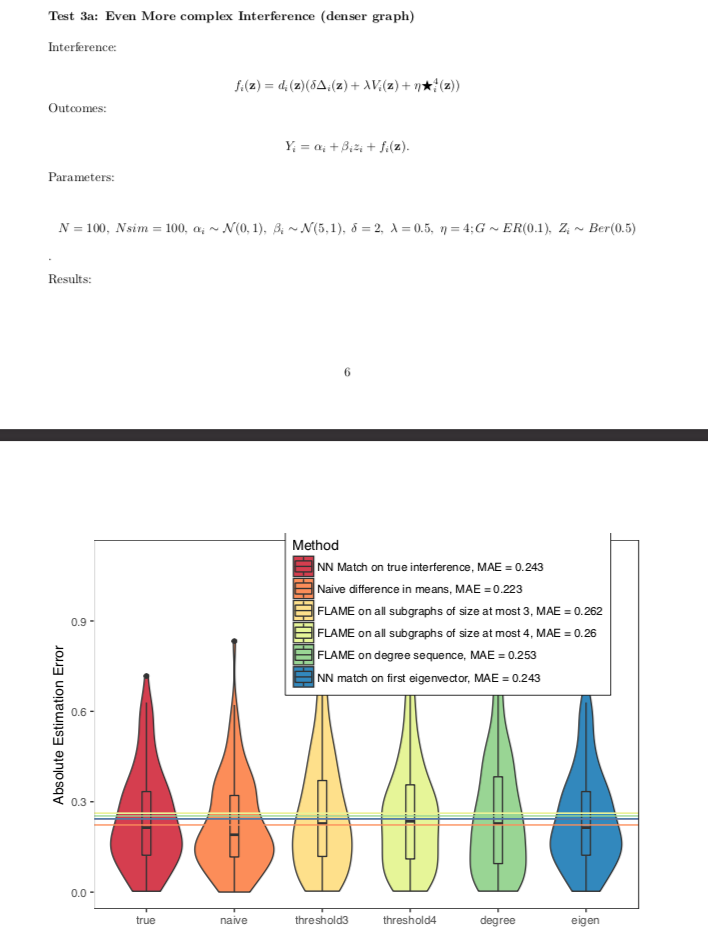
\includegraphics[height=3in]{even_more_complex.png}
\end{frame}
\begin{frame}{(OLD) Simulation Results}
\centering
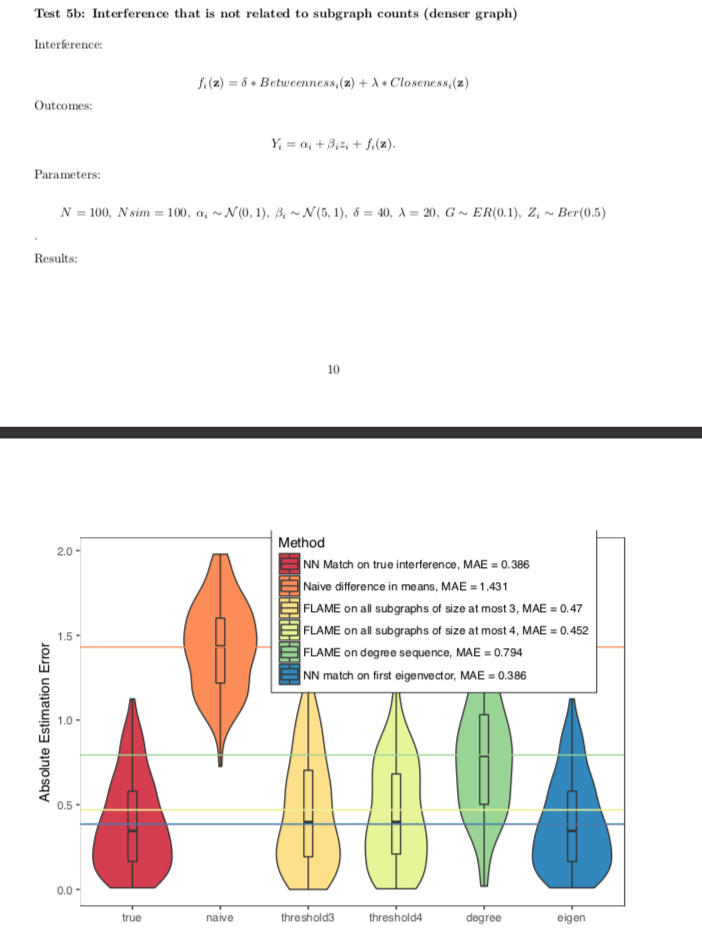
\includegraphics[height=3in]{unrelated_dense.png}
\end{frame}
% \begin{frame}{Bias Bound for oracle AME}
% As a preliminary result we can say that, under all the assumptions made before, with the true value of $\btheta$ and $S$ known, and if we choose a match for unit $i$ with treated neighborhood graph $g$ such that:
% \begin{align*}
% j \in {\tt MG(g)} \text{ if } j \in \argmin_{j = 1, \dots, n, T_j = 0} |\btheta^TS(g) - \btheta^TS(\Gnj)|,
% \end{align*}
% then the bias for the CATT of $i$ can be upper bounded by:
% \begin{align*}
% |\E[Y_i - Y_j] - \tau_i| &\leq K_1\sum_{h \in \mathcal{G}}|\btheta^TS(g) - \btheta^TS(h)|\frac{exp(\btheta^TS(h))}{\sum_{\ell \in \mathcal{G}}exp(\btheta^TS(\ell))}\\
% &\times\left[\sum_{d = S(g) - |S(g) - S(h)|}^{S(g) + |S(g) - S(h)|}\frac{D_{\btheta, S}(d)exp(d)}{\sum_{\ell \in \mathcal{G}}exp(\btheta^TS(\ell))}\right]^{n - 1}
% \end{align*}
% \end{frame}
\begin{frame}{Plan: We Want to Hit the October 8 AISTATS Deadline}
\begin{enumerate}
  \item We need to implement the revised $\tt PE$ function
  \item We need to redo the simulations
  \item More theory? Statements on how well the subgraph count can ``encode'' a given graph would be nice
  \item Find a good application
  \item Write!
\end{enumerate}
\end{frame}
\end{document}




